% graphic source: https://docs.google.com/presentation/d/11NBuIXM8JQMI2pnPQOirfBzwYOAdVX4sol6ymvlcvqA
\begin{figure}
\begin{minipage}{0.65\linewidth}
\begin{subfigure}{0.55\linewidth}
  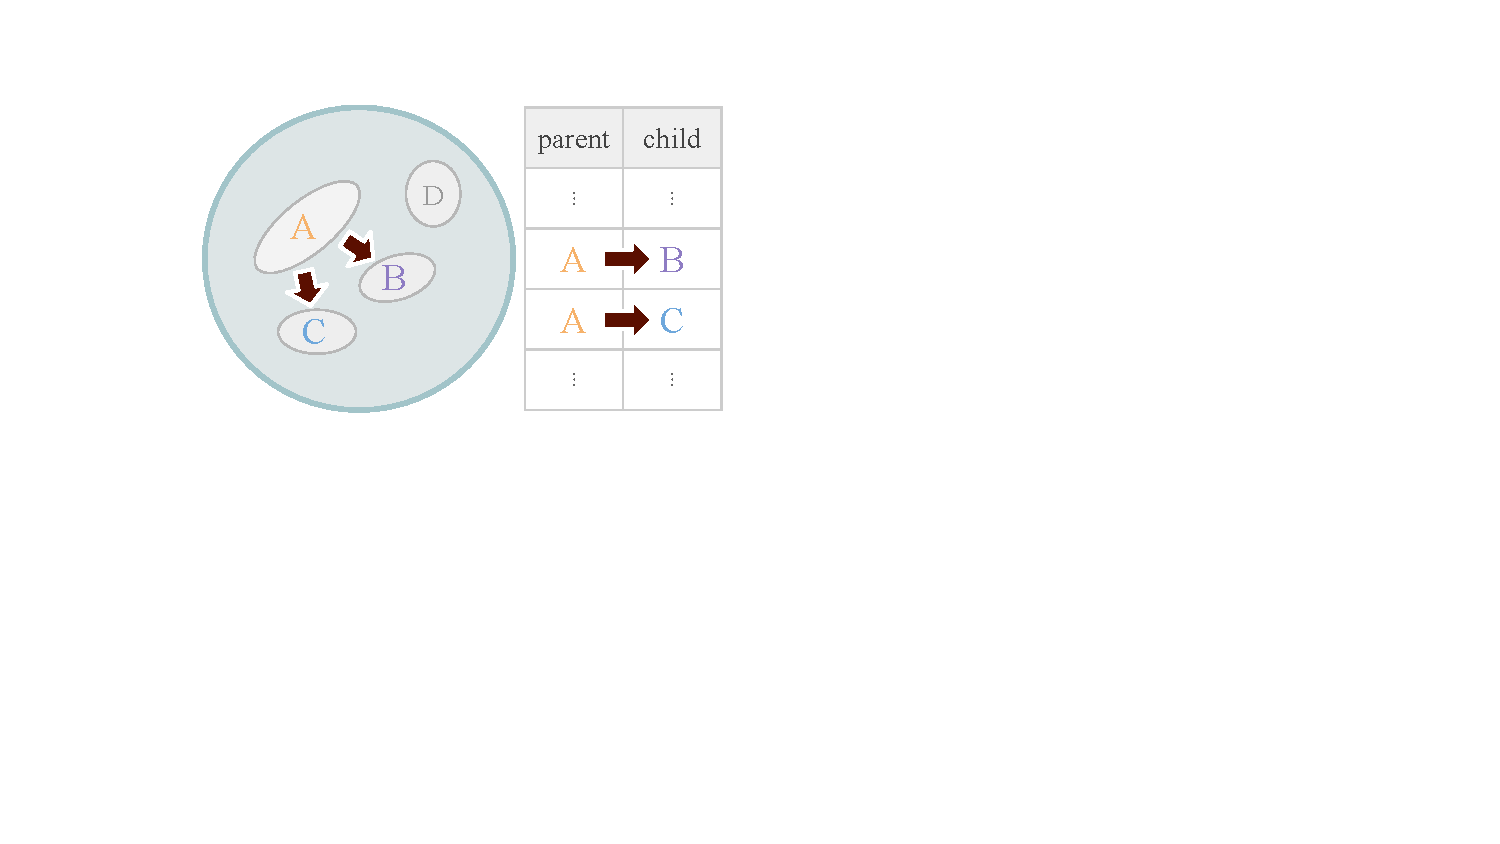
\includegraphics[width=\linewidth]{img/tracking-schematic}
  \caption{\footnotesize tracking approach}
  \label{fig:tracking-vs-reconstruction-schematic:tracking}
\end{subfigure}%
\begin{subfigure}{0.025\linewidth}~\end{subfigure}%
\vrule
\begin{subfigure}{0.025\linewidth}~\end{subfigure}%
\begin{subfigure}{0.35\linewidth}
  \centering
  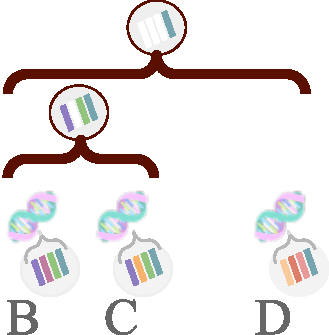
\includegraphics[width=\linewidth]{img/reconstruction-schematic}
  \caption{\footnotesize reconstruction approach}
  \label{fig:tracking-vs-reconstruction-schematic:reconstruction}
\end{subfigure}%
\begin{subfigure}{0.02\linewidth}~\end{subfigure}%
\end{minipage}%
\begin{minipage}{0.35\textwidth}
  \caption{%
  \textbf{Phylogeny tracking versus reconstruction.}
  \footnotesize
  TODO.
  }
  \label{fig:tracking-vs-reconstruction-schematic}
\end{minipage}
\end{figure}
